\documentclass[11pt, a4paper]{article}
\usepackage[a4paper, top=20mm, left=18mm, right=18mm, bottom=20mm]{geometry}
\usepackage{hyperref}
\usepackage[sf]{titlesec}
\usepackage{listings}
\usepackage{graphicx}
\usepackage{float}
\usepackage{caption}
\captionsetup{font={sf}}
\usepackage{color}
\hypersetup{hidelinks = true}
\definecolor{codegrey}{rgb}{0.95, 0.95, 0.96}
\lstset{backgroundcolor = \color{codegrey}, basicstyle=\normalsize\ttfamily}
\begin{document}
{\fontfamily{cmss}\selectfont

\title{\vspace{-20mm}CMPUT 291 - Mini Project 2 Design Document}
\date{}
\maketitle
\vspace{-20mm}

\section{Overview and User Guide}\label{OV}
The following software package is comprised of 3 phases. Phase 1 takes email data from an XML file and outputs the data into four files: terms.txt, emails.txt, dates.txt, and recs.txt. Phase 2 sorts these files and builds four indexes. Phase 3 is responsible for data retrieval, and queries the data.

\begin{figure}[H]
\centering
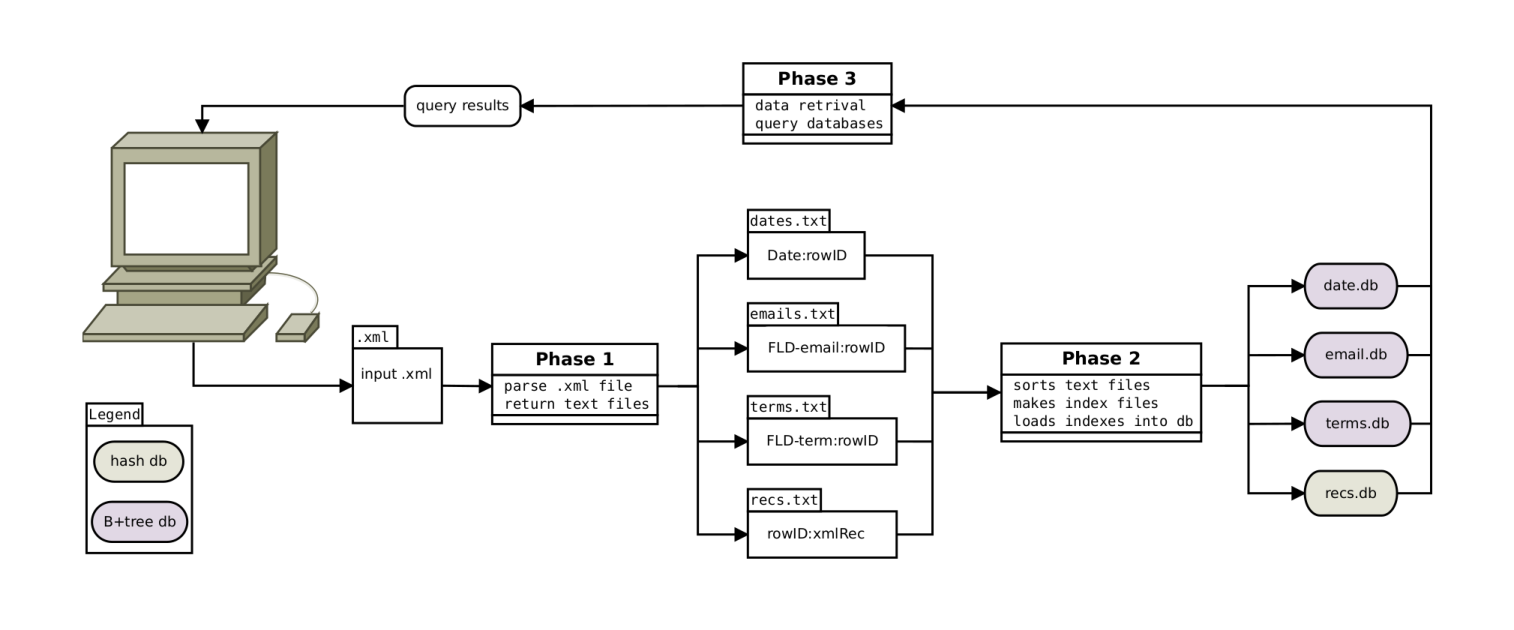
\includegraphics[width = \textwidth]{software_FD.pdf}\label{fig}
\caption{Flow diagram of files, data, and different phases of the software. For more implementation details see \emph{\nameref{SD}}.}
\end{figure}

\subsection{Phase 1: Preparing Data Files}
Preparation of the data files is completed by the python program \texttt{phase1.py}. The software reads in an \texttt{.xml} file specified by the user line by line, parses the line, and writes the data into four output files: \texttt{terms.txt}, \texttt{emails.txt}, \texttt{dates.txt}, and \texttt{recs.txt}. The phase 1 software can be run by entering the following command in the Linux terminal:
\begin{lstlisting}
    $ python3 phase1.py
\end{lstlisting}
The program will prompt the user to enter an \texttt{.xml} file:
\begin{lstlisting}
    Enter .xml file: datafile.xml
\end{lstlisting}
If the provided file is not found, or an incorrect file extension is given, an error message will display, and the user can re-enter a filename. If no extension is specified, the program will assume it is \texttt{.xml}. If the output files already exist in the directory, the program will overwrite the data currently on the files.

\subsection{Phase 2: Building Indexes}
Phase 2 takes the output files from phase 1 and sorts them, and produces four index files from the sorted data: \texttt{te.idx}, \texttt{em.idx}, \texttt{da.idx}, \texttt{re.idx}. If the index files already exist from a previous run, the data on them will be overwritten.

The index files are then loaded into four databases: \texttt{terms.db}, \texttt{email.db}, \texttt{date.db}, \texttt{recs.db}. Once again, if these databases are already found in the directory, they will be overwritten by the new data. 

No user input is required for phase 2. To build the indexes, simply execute the following command in the terminal:
\begin{lstlisting}
    $ python3 phase2.py
\end{lstlisting}
\subsection{Phase 3: Data Retrieval}
Phase 3 provides the user a simple interface to query the data prepared in phases 1 and 2. The query program uses \emph{Berkeley DB} to process the queries entered by the user. The user can query dates, emails, or terms. Depending on the type of query, it will have different formats. In general, queries are of the form:
\begin{lstlisting}
    > prefix:query
\end{lstlisting}

A date query will return all emails with dates that satisfy the query.
\begin{lstlisting}
    > date(:|>|<|>=|<=)YYYY/MM/DD
\end{lstlisting}

An email query returns all emails sent to/from/cc/bcc the email address specified:
\begin{lstlisting}
    > (to|from|cc|bcc):email@address.com
\end{lstlisting}

A term query returns all records that have the term in their subject or body field (field specified by user)
\begin{lstlisting}
    > (subj|body):term
\end{lstlisting}

Terms can also be queried without specifying the field. For example,
\begin{lstlisting}
    > confidential%
\end{lstlisting}
will return all records that have a term with prefix \emph{confidential} in their subject or body fields (confidential, confidentially, confidentiality, etc.).
 
The program will ignore all white spaces in the entered queries, so
\begin{lstlisting}
    > subj :   gas        body:earning
\end{lstlisting}
will successfully search the data for records that have gas in their subject and earning in their body fields. All queries are case-insensitive as well.

\section{Software Design}\label{SD}

\section{Testing Strategy}\label{TS}

\section{Group Work}\label{GW}


\end{document}
